\newpage
\chapter{Сложение моментов}
\par Пусть есть 2 слабовзаимодействующие системы с соответствующими моментами импульса, квантовыми числами и волновыми функциями:
\begin{table}[h]
\centering
\begin{tabular}[c]{|c|c|}
\hline 
1 подсистема & 2 подсистема \\ \hline 
$\hat{\vec{L}}^2_1$ и $\hat{\vec{L}}_{z1}$ & $\hat{\vec{L}}^2_2$ и  $\hat{\vec{L}}_{z2}$,\\
$L_1$ и $M_1$ & $L_2$ и $M_2$ \\
$\varphi_1(q_1)$ & $\varphi_2(q_2)$ \\
\hline
\end{tabular}
\end{table}
\par Масштаб для каждой из подсистем - расстояние между уровнями дискретного спектра. При взаимодействии уровни расходятся, появляются матричные элементы взаимодействия  $V_{nm}<< E_n -E_m$. Как сложить эти моменты? Можем определить оператор суммы и его квадрат, проекцию на $Oz$ (это направление не выделено, пространство изотропно, поэтому можно найти проекцию на совершенно любую ось): $\left(\hat{\vec{L}}_1 +\hat{\vec{L}}_2 \right)^2$. Тогда волновая функция $\varphi_{l_1, l_2, m_1, m_2}$ имеет $(2l_1+1)(2l_2+1)$ значений. Хотим перенумеровать, т.е. определить индексы, содержащие индексы полного момента.
$$\hat{\vec{L}}^2_1,\; \hat{\vec{L}}^2_{z2},\; \hat{\vec{L}}^2_1,\; \hat{\vec{L}}^2_{z2} \longrightarrow \varphi_{l_2l_2lm}$$
\par Причем $\varphi= \varphi_1(q_1) \cdot \varphi_2(q_2)$.
\par \textit{Небольшое отступление. Если $\hat{H}=\hat{H_1}(q_1)+\hat{H_2}(q_2)$, то УШ допускает разделение переменных: $\left( \hat{H_1}(q_1)+\hat{H_2}(q_2)\right)\varphi_1(q_1) \cdot \varphi_2(q_2) = E \varphi_1(q_1) \cdot \varphi_2(q_2) $ и соответственно $$\frac{\hat{H_1}(q_1)}{\varphi_1(q_1)} +\frac{\hat{H_2}(q_2)}{ \varphi_2(q_2)} = E$$
}
\par Можем сложить проекции моментов $\left(-i \hbar \frac{\partial}{\partial \varphi} \right)$.

\begin{table}[h]
\centering
\begin{tabular}[c]{|c|c|c|}
\hline 
M_1 & M_2 & M \\ \hline 
l_1 & l_2 & l_1+l_2\\
\begin{equation*}
 \begin{cases}
    l_1-1
\\
    l_1 
 \end{cases}
\end{equation*} & \begin{equation*}
 \begin{cases}
    l_2
\\
    l_2-1 
 \end{cases}
\end{equation*}&\begin{equation*}
 \begin{cases}
    l_1+l_2-1
\\
     l_1+l_2-1
 \end{cases}
\end{equation*}\\
...& ...& ...\\
\hline
\end{tabular}
\end{table}
\par Получается, одному значению суммарной проекции момента импульса могут соответствовать разные комбинации значений проекций моментов подсистем. При уменьшении $M$ таких комбинаций будет все больше.

\par 
\begin{wrapfigure}[10]{c}{0.45\linewidth} 
\vspace{-2ex}
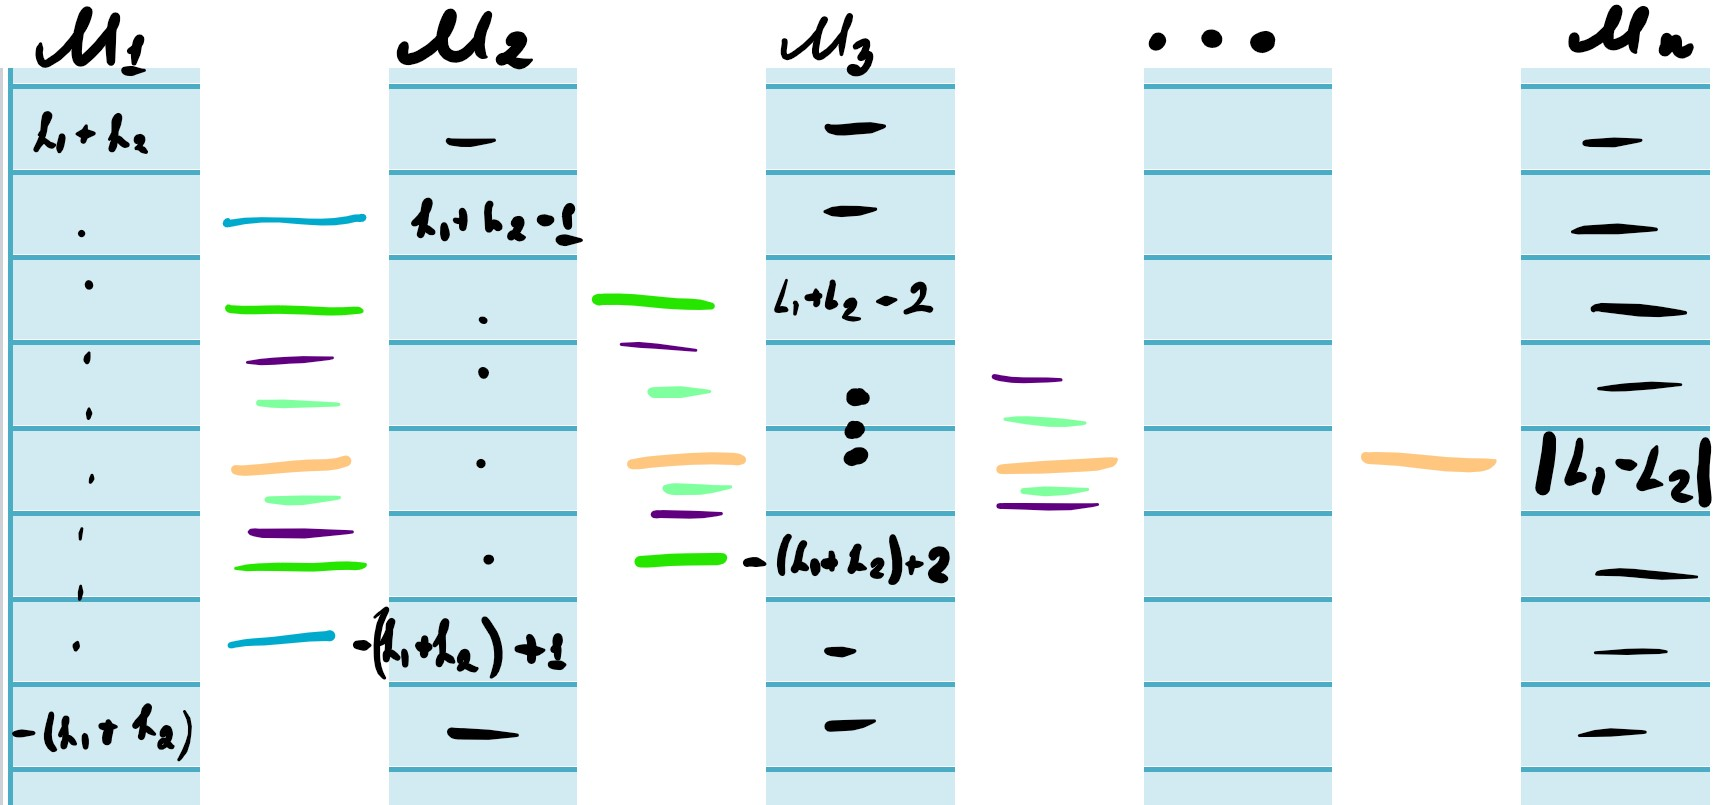
\includegraphics[width=1\linewidth]{pictures/18.1.jpg}
\caption{Увеличивающееся число комбинаций}
\end{wrapfigure}
\par Причем их число будет увеличиваться до тех пор, пока не останется суммарное значение $|l_1-l_2|$. Итого $l = \{ l_1+l_2,l_1+l_2-1, ..., |l_1-l_2|  \}$.
\par Итоговая четность состояния $(-1)^{l_{\sum}}$.